\begin{minipage}{0.75\linewidth}
\begin{figure}[h]
    \centering
    \begin{adjustbox}{max width=1.0\linewidth, keepaspectratio}
        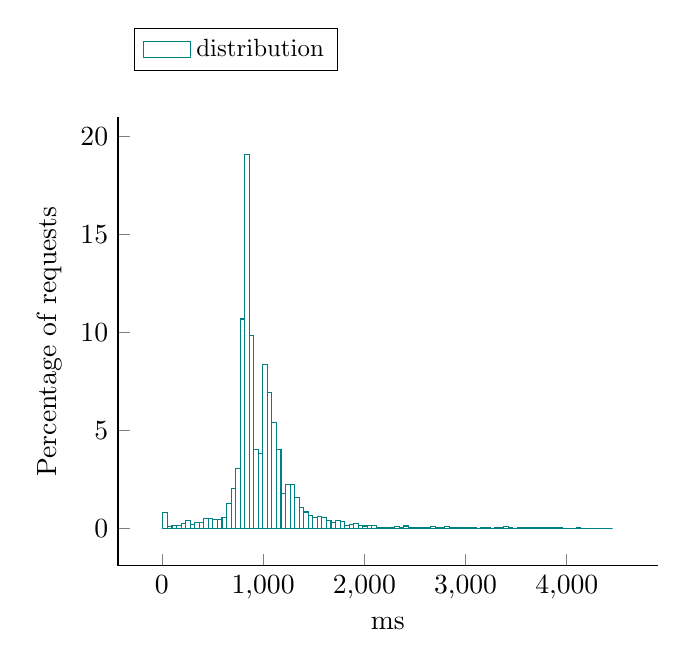
\begin{tikzpicture}
            \begin{axis}[ylabel = Percentage of requests, 
xlabel = ms, 
legend style = {nodes={scale=0.9, transform shape}, at={(0.03,1.2)}, anchor=north west, draw=black, fill=white, align=left, legend columns=3},
area style, mark size = 0pt,
 cycle list name = exotic,
  axis lines* = left]
		\addplot +[ybar interval] coordinates {
			 (10, 0.788478)
			 (54.88, 0.0735913)
			 (99.76, 0.136669)
			 (144.64, 0.147183)
			 (189.52, 0.262826)
			 (234.4, 0.388982)
			 (279.28, 0.210261)
			 (324.16, 0.315391)
			 (369.04, 0.315391)
			 (413.92, 0.515139)
			 (458.8, 0.504626)
			 (503.68, 0.441548)
			 (548.56, 0.452061)
			 (593.44, 0.546678)
			 (638.32, 1.26156)
			 (683.2, 2.0185)
			 (728.08, 3.03827)
			 (772.96, 10.6812)
			 (817.84, 19.0706)
			 (862.72, 9.85071)
			 (907.6, 4.02649)
			 (952.48, 3.81623)
			 (997.36, 8.37889)
			 (1042.24, 6.91758)
			 (1087.12, 5.39319)
			 (1132, 4.00547)
			 (1176.88, 1.79773)
			 (1221.76, 2.24979)
			 (1266.64, 2.23928)
			 (1311.52, 1.58747)
			 (1356.4, 1.06182)
			 (1401.28, 0.83053)
			 (1446.16, 0.672834)
			 (1491.04, 0.546678)
			 (1535.92, 0.599243)
			 (1580.8, 0.557191)
			 (1625.68, 0.410008)
			 (1670.56, 0.315391)
			 (1715.44, 0.388982)
			 (1760.32, 0.336417)
			 (1805.2, 0.147183)
			 (1850.08, 0.210261)
			 (1894.96, 0.231287)
			 (1939.84, 0.136669)
			 (1984.72, 0.115643)
			 (2029.6, 0.136669)
			 (2074.48, 0.136669)
			 (2119.36, 0.0630782)
			 (2164.24, 0.0315391)
			 (2209.12, 0.0315391)
			 (2254, 0.0210261)
			 (2298.88, 0.10513)
			 (2343.76, 0.0210261)
			 (2388.64, 0.115643)
			 (2433.52, 0.0630782)
			 (2478.4, 0.0210261)
			 (2523.28, 0.0315391)
			 (2568.16, 0.0315391)
			 (2613.04, 0.0525652)
			 (2657.92, 0.0735913)
			 (2702.8, 0.0630782)
			 (2747.68, 0.0420521)
			 (2792.56, 0.0735913)
			 (2837.44, 0.0210261)
			 (2882.32, 0.0210261)
			 (2927.2, 0.0210261)
			 (2972.08, 0.0420521)
			 (3016.96, 0.0210261)
			 (3061.84, 0.0210261)
			 (3106.72, 0)
			 (3151.6, 0.0210261)
			 (3196.48, 0.0420521)
			 (3241.36, 0.010513)
			 (3286.24, 0.0315391)
			 (3331.12, 0.0420521)
			 (3376, 0.0735913)
			 (3420.88, 0.0420521)
			 (3465.76, 0.010513)
			 (3510.64, 0.0210261)
			 (3555.52, 0.0315391)
			 (3600.4, 0.0315391)
			 (3645.28, 0.0525652)
			 (3690.16, 0.0420521)
			 (3735.04, 0.0630782)
			 (3779.92, 0.0210261)
			 (3824.8, 0.0315391)
			 (3869.68, 0.0420521)
			 (3914.56, 0.0315391)
			 (3959.44, 0.010513)
			 (4004.32, 0)
			 (4049.2, 0)
			 (4094.08, 0.0315391)
			 (4138.96, 0.010513)
			 (4183.84, 0.010513)
			 (4228.72, 0.010513)
			 (4273.6, 0)
			 (4318.48, 0)
			 (4363.36, 0.010513)
			 (4408.24, 0)
			 (4453.12, 0.010513)
		};
\addlegendentry{distribution};
           \end{axis}
      \end{tikzpicture}
  \end{adjustbox}
  \caption{Response time distribution - req = ReadUser-2}
\end{figure}
\end{minipage}\hfill\begin{minipage}{0.18\linewidth}
\begin{table}[h]
\begin{tabular}{|cc|}
\hline
\textbf{} & \textbf{ms}\\ \hline
 \Xhline{0.005\arrayrulewidth}
min & 10\\
 \Xhline{0.005\arrayrulewidth}
max & 4498\\
 \Xhline{0.005\arrayrulewidth}
mean & 997\\
 \Xhline{0.005\arrayrulewidth}
std & 390\\
\hline
\hline
 \Xhline{0.005\arrayrulewidth}
25th & 824\\
 \Xhline{0.005\arrayrulewidth}
50th & 899\\
 \Xhline{0.005\arrayrulewidth}
75th & 1094\\
 \Xhline{0.005\arrayrulewidth}
80th & 1135\\
 \Xhline{0.005\arrayrulewidth}
85th & 1212\\
 \Xhline{0.005\arrayrulewidth}
90th & 1314\\
 \Xhline{0.005\arrayrulewidth}
95th & 1572\\
 \Xhline{0.005\arrayrulewidth}
99th & 2756\\
\hline
\end{tabular}
\caption{Response time}
\end{table}
\end{minipage}\hfill